% The operate-and-improve loop for Ch28 ("Operating the Whole") — the Vol 3 / Design v1.0 capstone.
% Standalone TikZ; compiled by `book-scaffold build-figures` via pdflatex -> pdftocairo -> SVG.
% Clockwise cycle: production run -> see the failure (observability) -> make it an eval case ->
% fix it (bounded by cost/oversight/security) -> measure again -> back to production.
\documentclass[tikz,border=4mm]{standalone}
\usepackage{tikz}
\usetikzlibrary{positioning, arrows.meta, calc}

\begin{document}
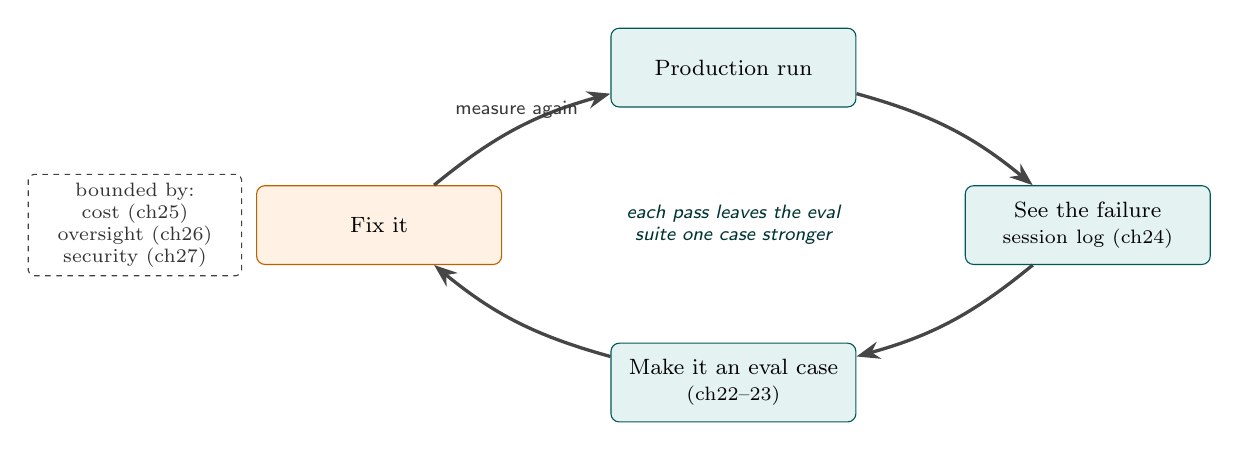
\begin{tikzpicture}[
  font=\sffamily,
  stage/.style={draw=teal!70!black, fill=teal!10, rounded corners=3pt, align=center,
    text width=2.9cm, minimum height=1.0cm, inner sep=3pt, font=\footnotesize},
  fix/.style={draw=orange!75!black, fill=orange!10, rounded corners=3pt, align=center,
    text width=2.9cm, minimum height=1.0cm, inner sep=3pt, font=\footnotesize},
  flow/.style={-Stealth, very thick, draw=gray!55!black},
  bound/.style={draw=gray!50!black, dash pattern=on 2pt off 2pt, rounded corners=2pt,
    align=center, inner sep=3pt, font=\scriptsize, text=gray!40!black}
]

% four stages in a clockwise diamond
\node[stage] (prod)  at (4.5,4)  {Production run};
\node[stage] (see)   at (9,2)    {See the failure\\{\scriptsize session log (ch24)}};
\node[stage] (evalc) at (4.5,0)  {Make it an eval case\\{\scriptsize (ch22--23)}};
\node[fix]   (fix)   at (0,2)    {Fix it};

% clockwise flow
\draw[flow] (prod)  to[bend left=12] (see);
\draw[flow] (see)   to[bend left=12] (evalc);
\draw[flow] (evalc) to[bend left=12] (fix);
\draw[flow] (fix)   to[bend left=12]
  node[pos=0.5, above, font=\sffamily\scriptsize, text=gray!45!black] {measure again} (prod);

% the fix is bounded by the other three surfaces
\node[bound, left=5pt of fix, text width=2.5cm] {bounded by:\\cost (ch25)\\oversight (ch26)\\security (ch27)};

% centre note
\node[align=center, font=\sffamily\scriptsize\itshape, text=teal!40!black, text width=3.3cm]
  at (4.5,2) {each pass leaves the eval suite one case stronger};

\end{tikzpicture}
\end{document}
